%! Author = Len Washington III
%! Date = 8/21/24

% Preamble
\documentclass[
	number={1},
	title={Machine Learning Fundamentals}
]{cs584notes}
\usepackage{amstex}

% Document
\begin{document}

\newcommand{\learningtask}[3]{%
	\begin{description}
	\item[$T$]: #1
	\item[$P$]: #2
	\item[$E$]: #3
	\end{description}
	\vspace*{0.25em}
}

\section{Machine Learning}\label{sec:machine-learning}
\begin{displayquote}
	``\emph{Learning} is any process by which a system improves \emph{performance} from \emph{experience}.'' -- Herbert Simon
\end{displayquote}

\textbf{Machine Learning} is the \emph{study of algorithms} that --
\begin{itemize}
	\item improve their performance \emph{$P$}
	\item at some task \emph{$T$}
	\item with experience \emph{$E$}.
\end{itemize}
A well-defined \emph{learning task} is given by \emph{$<P,T,E>$}.

\section{Defining Learning Tasks}\label{sec:defining-learning-tasks}
\learningtask{Playing checkers.}{Percentage of games won against an arbitrary opponent.}{Playing practice games against itself.}

\learningtask{Recognizing hand-written words.}{Percentage of words correctly classified.}{Database of human-labeled images of handwritten words.}

\learningtask{Driving on four-lane highways using vision sensors.}{Average distance traveled before a human-judged error.}{A sequence of images and steering commands recorded while observing a human driver.}

\learningtask{Categorize email messages as spam or legitimate.}{Percentage of email messages correctly classified.}{Database of emails, some with human-given labels.}

\section{Why we use ML?}\label{sec:why-we-use-ml?}
\begin{itemize}
	\item Human expertise does not exist (navigating on Mars).
	\item Humans can't explain their expertise (speech recognition).
	\item Models must be customized (personalized medicine).
	\item Models are based on huge amounts of data (genomics).
\end{itemize}

\section{Machine Learning Applications}\label{sec:machine-learning-applications}
\begin{itemize}
	\item Recognizing patterns:
	\begin{itemize}
		\item Facial identities or facial expressions.
		\item Handwritten or spoken words.
		\item Medical images.
	\end{itemize}
	\item Generating pattens:
	\begin{itemize}
		\item Generating images or motion sequences.
	\end{itemize}
	\item Recognizing anomalies:
	\begin{itemize}
		\item Unusual credit card transactions.
		\item Unusual patterns of sensor readings in a nuclear power plant.
	\end{itemize}
	\item Prediction:
	\begin{itemize}
		\item Future stock prices or currency exchange rates.
	\end{itemize}
\end{itemize}

\section{Datasets and Features}\label{sec:datasets-and-features}
\begin{itemize}
	\item A \emph{dataset} is a set of data grouped into a \emph{collection} with which developers can work to meet their goals.
	In a dataset, \emph{rows} represent the number of data points and \emph{columns} represent the features of the dataset.
	\item The \emph{features of a dataset} are the most \emph{critical aspect} of the dataset, as based on the features of each available data point, will there be any possibility of \emph{deploying models} to find the \emph{output to predict} the features of any new data point that may be added to the dataset.
\end{itemize}

\begin{figure}[H]
	\centering
	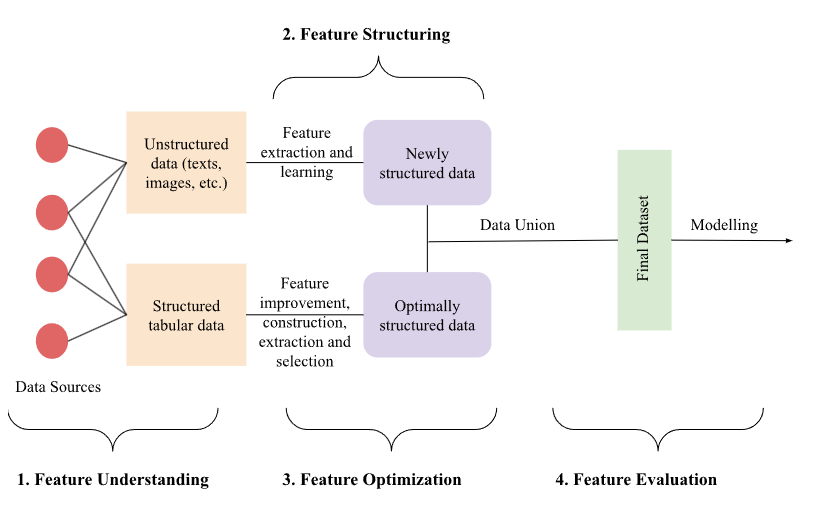
\includegraphics[width=\textwidth]{figures/1/datasets-and-features}
	\caption{Datasets and Features}
	\label{fig:datasets-and-features}
\end{figure}

\section{Feature Scaling}\label{sec:feature-scaling}
\emph{Scale} the data to a fixed range \data{$[0, 1]$}.
\begin{itemize}
	\item \definition{Normalization}{Rescale the \emph{data} \data{$x$} using the \emph{mean} \data{$(\mu)$} and the \emph{standard deviation} \data{$(\sigma)$} of the data.}
	\begin{equation}
		x_{norm} = \frac{x - \mu}{\sigma}
		\label{eq:normalization}
	\end{equation}
	\item \emph{Min-Max Scaling}:
	\begin{equation}
		x_{minmax} = \frac{x - x_{min}}{x_{max} - x_{min}}
		\label{eq:min-max-scaling}
	\end{equation}
\end{itemize}

\section{Types of Datasets}\label{sec:types-of-datasets}
\begin{itemize}
	\item Numerical Dataset.
	\item Categorical Dataset.
	\item Web Dataset.
	\item Time series Dataset.
	\item Image Dataset.
	\item Ordered Dataset.
	\item Bivariate Dataset.
	\item Multivariate Dataset.
\end{itemize}

\section{The Task, $T$}\label{sec:the-task}
Tasks are usually described in terms of how the machine learning should process an example: \data{$x \in \mathbb{R}^{n}$} where each entry \data{$x_{i}$} is a \emph{feature}.
\begin{description}[font=\color{emphblue}]
	\item[Classification:] Learn \data{$f: \mathbb{R}^{n}\rightarrow\{1,\dots,k\}$}
	\begin{itemize}
		\item \data{$y=f(x)$}: \emph{assigns input} to the \emph{category} with \emph{output} \data{$y$}.
		\item Example: Object recognition
	\end{itemize}
	\item[Regression:] Learn \data{$f: \mathbb{R}^{n} \rightarrow \mathbb{R}$}
	\begin{itemize}
		\item Example: Weather prediction, real estate price prediction.
	\end{itemize}
	\item[Transcription:] \emph{Unstructured representation} to \emph{discrete textual form}.
	\begin{itemize}
		\item Example: Optical character recognition, speech recognition.
	\end{itemize}
	\item[Machine translation:] Sequence to sequence.
	\begin{itemize}
		\item Example: Translate English to French.
	\end{itemize}
	\item[Synthesis and sampling:] \emph{Generate examples} that are \emph{similar} to those in the \emph{training data}.
	\begin{itemize}
		\item Example: Generate textures for video games, speech synthesis.
	\end{itemize}
\end{description}

\section{The Experience, $E$}\label{sec:the-experience-$e$}

\subsection{Supervised Learning}\label{subsec:supervised-learning}
\begin{itemize}
	\item Experience is a \emph{labeled dataset} (or data points).
	\item Each \emph{datapoint} has a \emph{label} or target.
	\item Given \data{$(x_{1}, y_{1}), (x_{2}, y_{2}), \dots, (x_{n}, y_{n})$}, learn a \emph{function} \data{$f(x)$} to predict $y$ given $x$
	\begin{itemize}
		\item \data{$y$} is real-valued == \emph{regression}
		\item \data{$y$} is categorical == \emph{classification}
	\end{itemize}
\end{itemize}

\subsection{Unsupervised learning}\label{subsec:unsupervised-learning}
\begin{itemize}
	\item Experience is an \emph{unlabeled dataset}.
	\item Clustering, learning probability distribution, denoising, etc.
\end{itemize}

\subsection{Reinforcement learning}\label{subsec:reinforcement-learning}
\begin{itemize}
	\item Experience is the interaction with an \emph{environment}.
\end{itemize}

\subsection{Transfer Learning}\label{subsec:transfer-learning}
A model trained off of dataset $D_{1}$ can be retrained with dataset $D_{2}$ to add more knowledge to the model.
This means that a model does not have to be trained from scratch.

\section{Performance Measure, $P$}\label{sec:performance-measure-$p$}
\begin{description}[font=\color{emphblue}]
	\item[Accuracy:] The \emph{proportion} of examples for which the \emph{model produces} the \emph{correct output}.
	\item[Error rate:] The \emph{proportion} of examples for which the \emph{model produces} an \emph{incorrect output}.
	\item[Loss function:] Quantifies the \emph{difference} between the \emph{predicted outputs} of a machine learning algorithm and the \emph{actual target values}.
	\item[Generalization] Ability to \emph{perform well} on previously \emph{unobserved data}; e.g., \emph{evaluate} the \emph{performance} using a \emph{test set}.
\end{description}

\section{No Free Lunch Theorem}\label{sec:no-free-lunch-theorem}
\begin{itemize}
	\item \definition{``No Free Lunch Theorem''}{without having substantive information about the modeling problem, there is \emph{no single model} that will always \emph{do better than any other model}.}
	\item The \emph{goal} of machine learning research is not to seek a universal learning algorithm or the absolute best learning algorithm.
	\item Instead, our goal is to understand what kinds of distributions are relevant to the real world and what kinds of machine learning algorithms perform well on data drawn distributions we care about.
\end{itemize}

\section{Training and Testing}\label{sec:training-and-testing}
\begin{itemize}
	\item \definition{Training data}{used to \emph{train} the machine learning model}.
	\item \definition{Testing data}{used to determine the performance of the trained model.}
\end{itemize}

\subsection{Independent and Identically Distributed (IID) assumptions}\label{subsec:iid-assumptions}
\begin{itemize}
	\item Examples in each dataset are independent from each other
	\item Training and testing set are identically distributed; i.e., drawn from the same probability distribution as each other.
\end{itemize}

\section{Fitting}\label{sec:fitting}
\begin{itemize}
	\item \definition{Underfitting}{when the model is \emph{unable} to \emph{obtain} a sufficiently low training error value.}
	\item \definition{Overfitting}{when the \emph{gap} between the \emph{training error} and \emph{test error} is too large.}
	\item \definition{Hypothesis}{the machine's presumption regarding the connection between the input features and the output.}
\end{itemize}

Consider a \emph{hypothesis \data{$h$}} and its$\dots$
\begin{itemize}
	\item Error rate over training data: \data{$error_{train}(h)$}
	\item True error rate over all data: \data{$error_{true}(h)$}
\end{itemize}

Hypothesis \data{$h$} \emph{overfits} the training error if there is an alternative hypothesis \data{$h'$} such that
\begin{equation}
\begin{aligned}
	error_{train}(h) &< error_{train}(h')\\
	error_{true}(h) &> error_{true}(h')
\end{aligned}\label{eq:hypothesis}
\end{equation}

\subsection{Resolving Underfitting}\label{subsec:resolving-underfitting}
\begin{itemize}
	\item \emph{Increasing} model \emph{complexity}.
	\item Using a different ML \emph{algorithm}.
	\item Increasing the amount of \emph{training data}.
	\item \emph{Ensemble methods} to combine multiple methods to create better outputs.
	\item \emph{Feature engineering} for \emph{creating new model features} from the existing ones that may be more relevant to the learning task.
\end{itemize}

\subsection{Resolving Overfitting}\label{subsec:resolving-overfitting}
\begin{itemize}
	\item \definition{Cross-Validation}{a technique for evaluating ML models by \emph{training several ML models} on \emph{subsets} of the available input data and evaluating them on another subset of the data.}
	\item \definition{Regularization}{a technique where a \emph{penalty term} is added to the \emph{loss function}, discouraging the model from assigning too much importance to individual features.}
	\item \definition{Early-stopping}{stops training when a monitored \emph{metric} has \emph{stopped improving}.}
	\item \definition{Bagging}{\emph{learning multiple models} in parallel and applying \emph{majority voting} to choose the final candidate model.}
\end{itemize}

\section{Cross-Validation}\label{sec:cross-validation}
\subsection{\data{$k$}-\emph{fold} cross-validation}\label{subsec:k-fold-cross-validation}
\begin{itemize}
	\item Divide data into \data{$k$} \emph{folds}.
	\item Train on \data{$k-1$} \emph{folds}, use the \data{$k^{\mbox{th}}$} to \emph{measure error}.
	\item Repeat \data{$k$} \emph{times}; use \emph{average error} to measure generalization accuracy.
	\item Statistically valid and gives good accuracy estimates.
\end{itemize}

\begin{figure}[H]
	\centering
	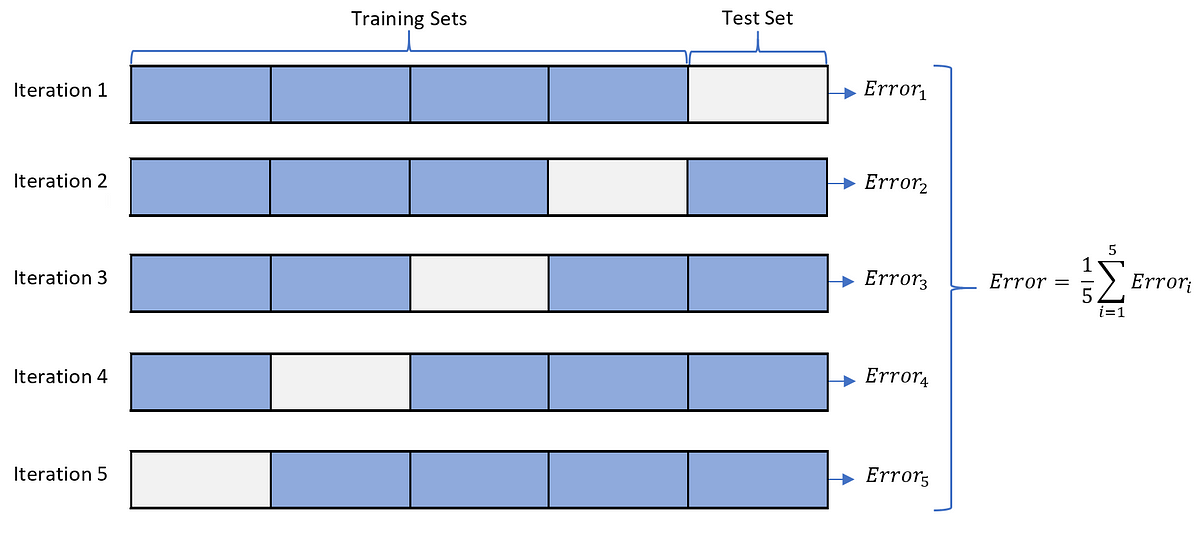
\includegraphics[width=\textwidth]{figures/1/k-fold-cross-validation}
	\caption{\data{$k$-fold Cross-Validation}}
	\label{fig:k-fold-cross-validation}
\end{figure}

\subsection{\emph{Leave-one-out} cross validation (LOOCV)}\label{subsec:loocv}
\begin{itemize}
	\item \data{$k$}-\emph{fold} cross validation with \data{$k=N$}, where \data{$N$} is the number of \emph{data points}.
	\item Quite accurate, but also \emph{expensive}, since it requires \emph{building} \data{$N$} \emph{models}.
\end{itemize}

\begin{figure}[H]
	\centering
	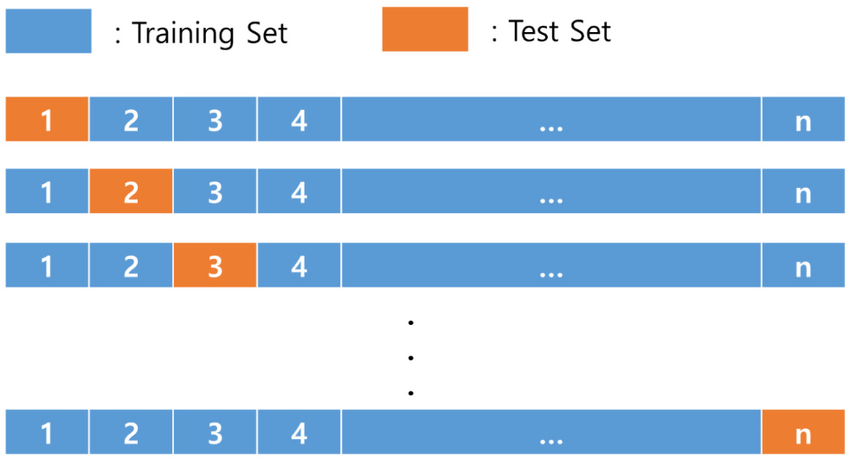
\includegraphics[width=\textwidth]{figures/1/loocv}
	\caption{LOOCV}
	\label{fig:loocv}
\end{figure}

\section{Parametric Learning}\label{sec:parametric-learning}
\definition{Parametric learning algorithms}{make \emph{strong assumptions} about the form of the \emph{mapping function} between the input features and output.}
\begin{itemize}
	\item For example, logistic regression, linear regression, perceptron, \naive bayes, neural network.
	\item \emph{Benefits} of such models are
	\begin{enumerate}[label=(\alph*)]
		\item easier to understand and interpret results
		\item very fast to learn from data
		\item do not require as much training data
		\item can work even if they do not fit the data perfectly.
	\end{enumerate}
	\item However, by pre-emptively choosing a functional form, these methods are highly constrained to the specified form.
\end{itemize}

\section{Non-parametric Learning}\label{sec:non-parametric-learning}
\definition{Non-parametric learning algorithms}{\emph{do not make assumptions} about the form of the \emph{mapping function} between the input features and output.}
\begin{itemize}
	\item For example, SVM, $k$-NN, $k$-means, decision tree.
	\item \emph{Benefits} include
	\begin{enumerate}[label=(\alph*)]
		\item being capable of fitting a large number of functional forms,
		\item there are no assumptions about the underlying$\dots$,
		\item can result in higher performance models for prediction.
	\end{enumerate}
	\item However,
	\begin{enumerate}[label=(\alph*)]
		\item it requires a lot more training date,
		\item takes longer to train,
		\item prone to overfitting.
	\end{enumerate}
\end{itemize}

\section{Model Selection}\label{sec:model-selection}
\begin{itemize}
	\item \emph{Adopting} the \emph{best algorithm} and model for a specific dataset by \emph{assessing} and \emph{comparing different models} to identify the one with the \emph{best results.}
\end{itemize}

\section{AIC/BIC}\label{sec:aic/bic}
\definition{\emph{Akaike Information Criterion} (AIC) and \emph{Bayesian Information Criterion} (BIC)}{compares different models to choose one that \emph{best fits the data}.}
\begin{itemize}
	\item The goal of both AIC and BIC is to \emph{balance} the \emph{goodness-of-fit} of the model with its \emph{complexity}, in order to avoid overfitting or underfitting.
	\item Both \emph{AIC} and \emph{BIC} \emph{penalize models} with \emph{large number of parameters} relative to the \emph{size} of the \emph{data}, but BIC penalizes more severely.
	\begin{equation}
		\begin{aligned}
			\min AIC &= \min\left\{ 2m - 2\log(L) \right\}\\
			\min BIC &= \min\left\{ m\log(n) - 2\log(L) \right\}
		\end{aligned}\label{eq:aic-bic}
	\end{equation}
	where \data{$m$} is the \emph{number} of \emph{model parameters}, \data{$n$} is the \emph{number} of \emph{data points}, and \data{$L$} is the \emph{maximum likelihood} of the model.
\end{itemize}

\begin{figure}[H]
	\centering
	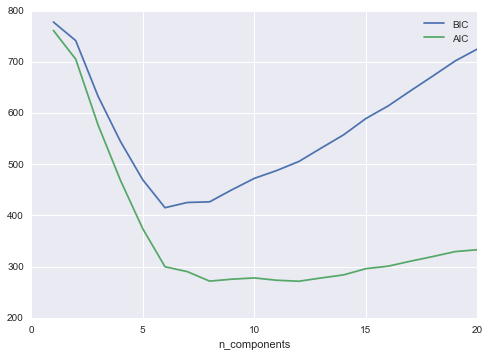
\includegraphics[width=\textwidth]{figures/1/aic_bic}
	\caption{AIC/BIC}
	\label{fig:aic-bic}
\end{figure}

\section{Classification}\label{sec:classification}

\emph{Predictive modeling} problem where a \emph{class label} is \emph{predicted} for a given example of input data.\\

Types of classification problems:
\begin{itemize}
	\item Binary classification.
	\item Multi-class classification.
	\item Multi-label classification.
	\item Imbalanced classification.
\end{itemize}

\begin{figure}[H]
	\centering
	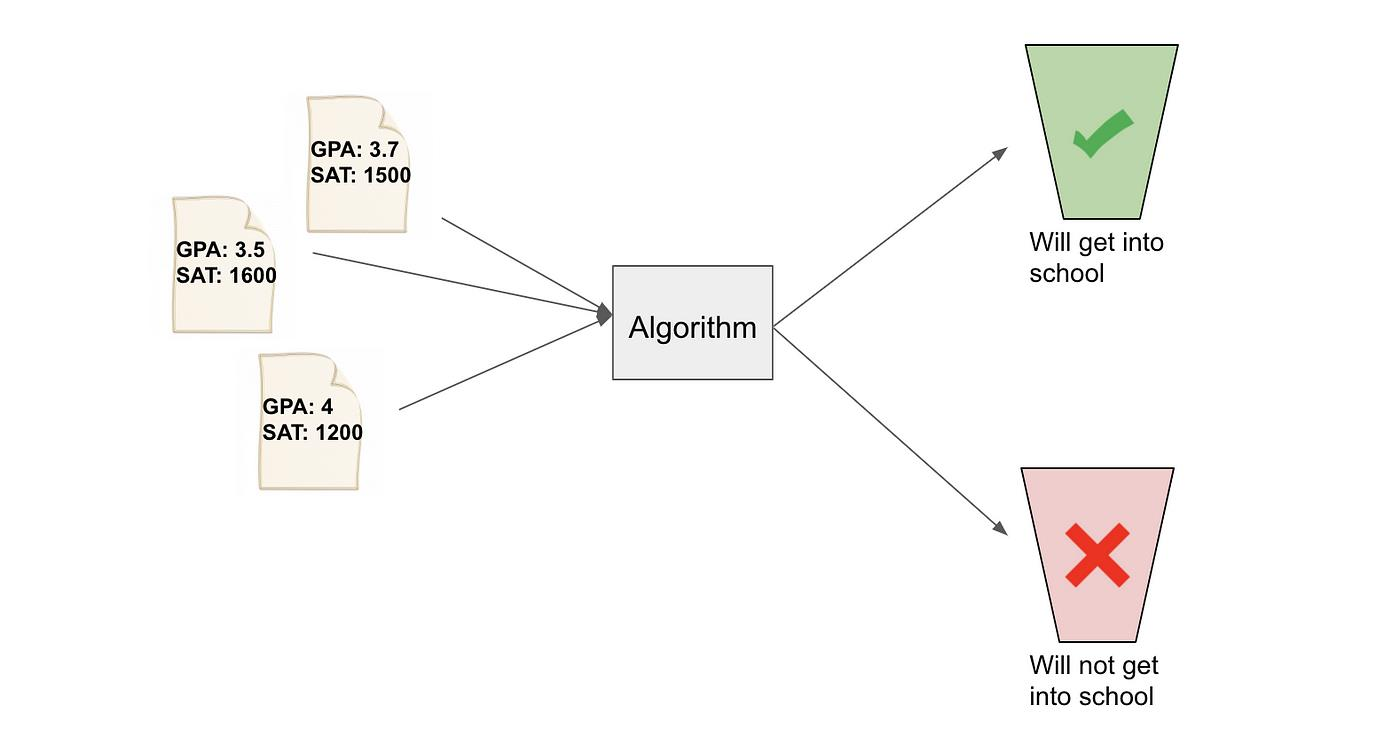
\includegraphics[width=\textwidth]{figures/1/binary_classification}
	\caption{Binary Classification}
	\label{fig:binary-classification}
\end{figure}

\begin{figure}[H]
	\centering
	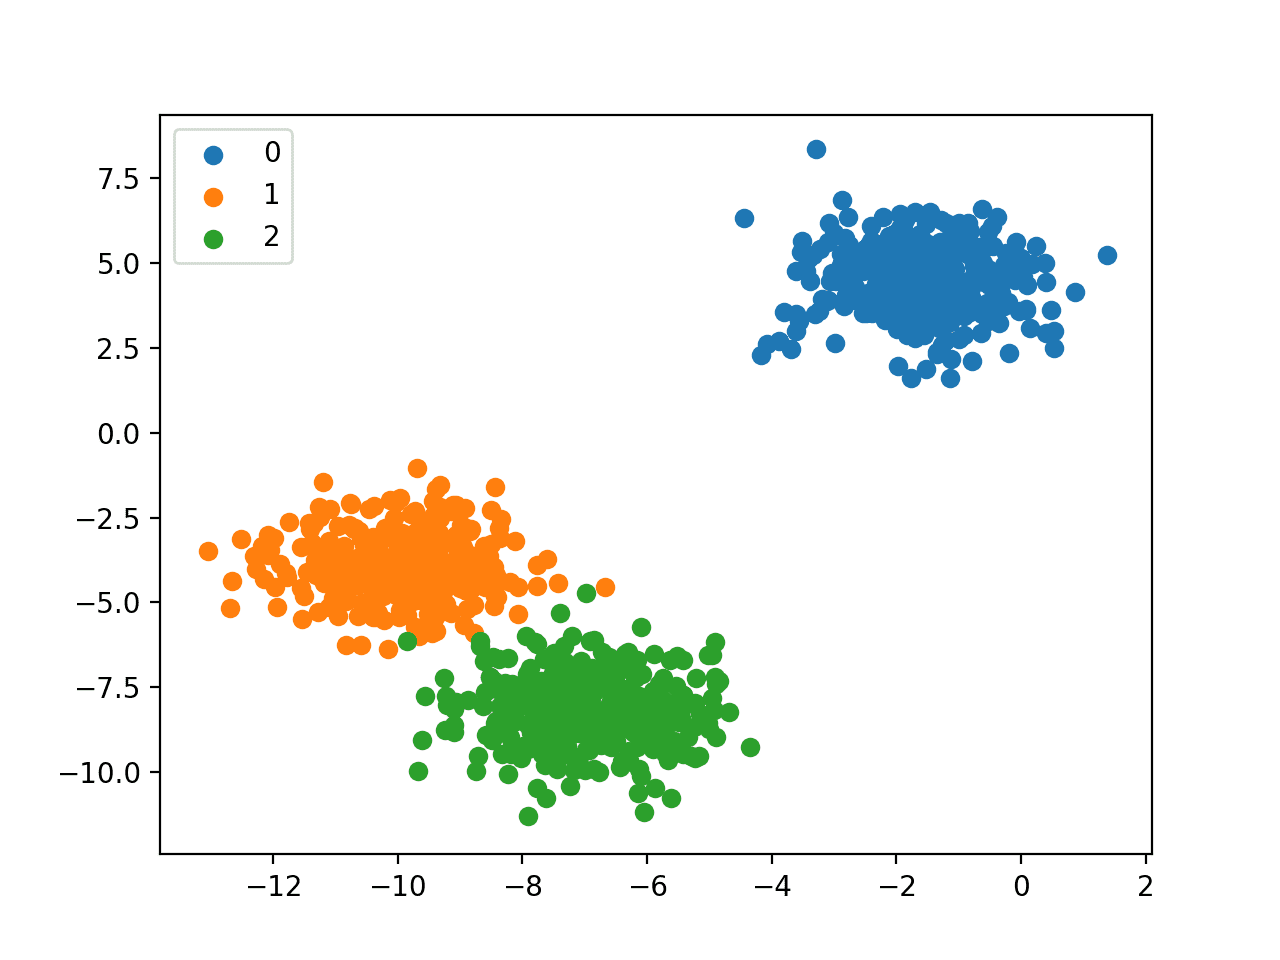
\includegraphics[width=\textwidth]{figures/1/multi_class_classification}
	\caption{Multi-class Classification}
	\label{fig:multi-class-classification}
\end{figure}

\begin{figure}[H]
	\centering
	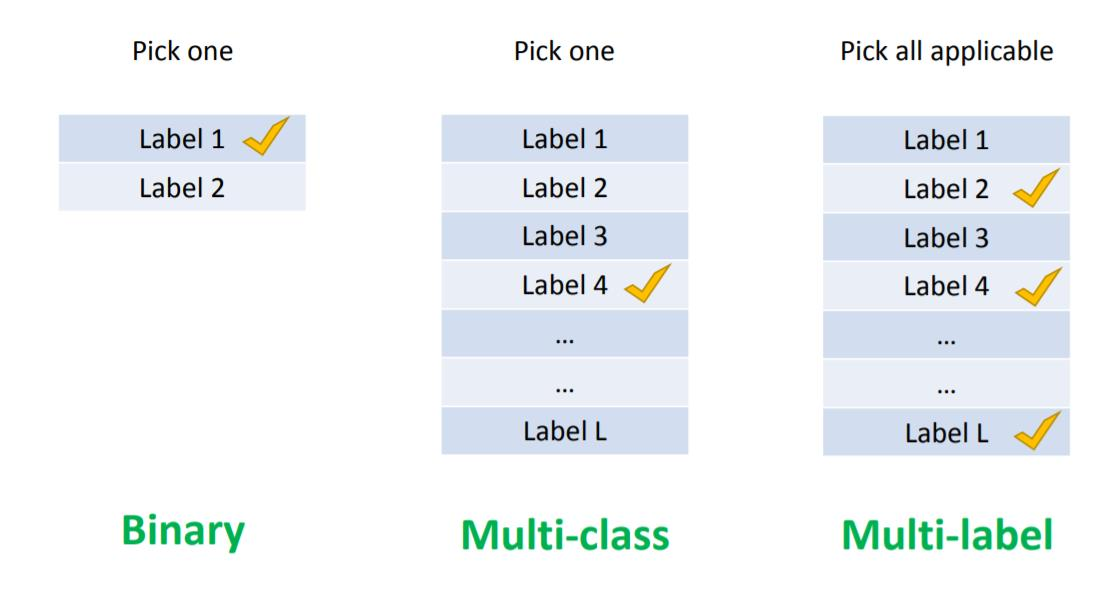
\includegraphics[width=\textwidth]{figures/1/multi_label_classification}
	\caption{Multi-label Classification}
	\label{fig:multi-label-classification}
\end{figure}

\begin{figure}[H]
	\centering
	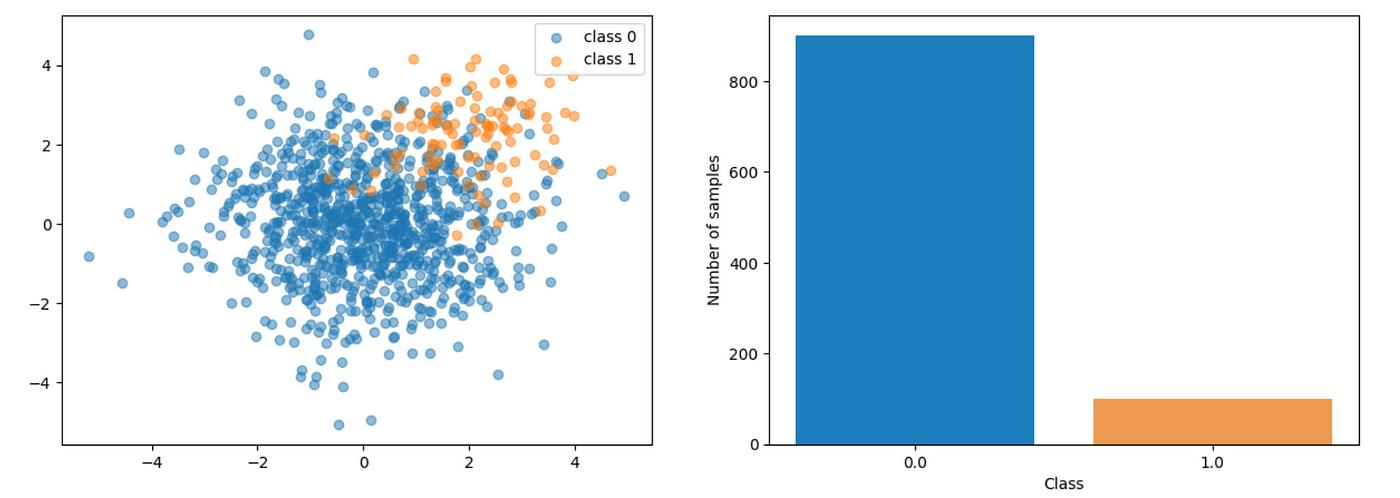
\includegraphics[width=\textwidth]{figures/1/imbalanced_classification}
	\caption{Imbalanced Classification}
	\label{fig:imbalanced-classification}
\end{figure}

\section{Classification Applications}\label{sec:classification-applications}
\begin{itemize}
	\item Medical diagnosis
	\begin{itemize}
		\item Features: age, gender, history, symptoms, test results.
		\item Label: disease.
	\end{itemize}
	\item Email spam detection
	\begin{itemize}
		\item Features: sender-domain, length, images, keywords.
		\item Label: spam or not-spam.
	\end{itemize}
	\item Credit card fraud detection
	\begin{itemize}
		\item Features: user, location, item, price.
		\item Label: fraud or legitimate.
	\end{itemize}
\end{itemize}

\begin{figure}[H]
	\centering
	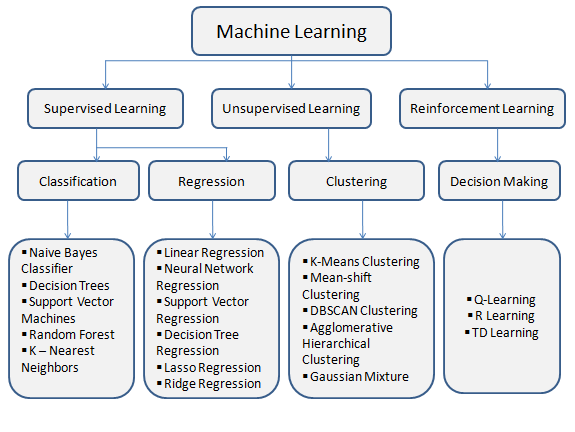
\includegraphics[width=\textwidth]{figures/1/ml_algorithm_tree}
	\caption{Machine Learning Algorithm Tree}
	\label{fig:ml_algorithm_tree}
\end{figure}


\end{document}
